\documentclass[10pt,a4paper]{article}
\usepackage[utf8]{inputenc}
\usepackage[ngerman]{babel}
\usepackage{url}
\usepackage[margin=2.5cm]{geometry}
\usepackage{graphicx}
\usepackage{caption}

% --- ERWEITERTE TIKZ-BIBLIOTHEKEN FÜR BESSERE SCHAUBILDER ---
\usepackage{tikz}
\usetikzlibrary{shapes.geometric, arrows.meta, positioning, fit, backgrounds, shapes.symbols}

% --- HYPERREF MUSS MEIST ZULETZT GELADEN WERDEN ---
\usepackage{hyperref}
\hypersetup{
colorlinks=true,
linkcolor=blue,
filecolor=magenta,
urlcolor=cyan,
pdftitle={Ausarbeitung zum Pipeline-Architekturstil},
pdfauthor={Alber Jonas, Schweitzer Tim},
pdfsubject={Softwarearchitektur},
pdfkeywords={Pipeline, Pipes and Filters, Architekturstil, Software Engineering},
bookmarks=true,
pdfpagemode=FullScreen,
}

% ---  TIKZ-STILE FÜR BESSERE LESBARKEIT ---
\tikzstyle{filter_node} = [rectangle, rounded corners, minimum height=1.2cm, text centered, draw=black, fill=blue!20, font=\small]
\tikzstyle{source_sink} = [ellipse, minimum height=1.2cm, text centered, draw=black, fill=red!20, font=\small]
\tikzstyle{tester_node} = [diamond, aspect=1.5, minimum height=1.2cm, text centered, draw=black, fill=orange!30, font=\small, inner xsep=0]
\tikzstyle{broker_node} = [cylinder, shape border rotate=90, aspect=0.5, minimum height=1.5cm, text centered, draw=black, fill=yellow!40, font=\small]
\tikzstyle{pipe_arrow} = [thick, -{Stealth[length=3mm, width=2mm]}]
\tikzstyle{pipe_label} = [font=\footnotesize, fill=white, inner sep=1pt]

\title{Ausarbeitung zum Pipeline-Architekturstil}
\author{Alber Jonas 15444427, Schweitzer Tim 29844429}
\date{\today}
\begin{document}

\maketitle

\begin{abstract}
\noindent % Verhindert Einzug
Der Pipeline-Architekturstil (Pipes-and-Filters) ist ein etabliertes Paradigma zur Strukturierung von Systemen in modulare, sequenzielle Verarbeitungsschritte. Aufgrund seiner konzeptionellen Einfachheit und Modularität eignet er sich besonders für datenflussorientierte Aufgaben.\cite{richards2020} Diese Ausarbeitung analysiert die Kernprinzipien dieses Stils, beleuchtet typische Anwendungsfelder und bewertet kritisch dessen Vor- und Nachteile. Ein besonderer Fokus liegt auf der Evolution von traditionellen, monolithischen Implementierungen hin zu modernen, verteilten Streaming-Paradigmen und den damit verbundenen neuen Herausforderungen. Die Untersuchung unterstreicht die anhaltende Relevanz des Musters für die Bewältigung komplexer Datenverarbeitungsaufgaben.
\end{abstract}

\section{Einführung und Historischer Kontext}
Der Pipeline-Architekturstil, auch als Pipes-and-Filters bekannt, zerlegt komplexe Funktionalität in eine Kette unabhängiger, sequenzieller Verarbeitungsschritte. Die Klarheit des Datenflusses macht ihn zu einer attraktiven Wahl für viele Probleme, insbesondere in der Datenverarbeitung. Trotz neuerer Architekturparadigmen hat der Stil seine Relevanz bewahrt und erlebt durch moderne Technologien eine Renaissance.

Die philosophische Grundlage ist das Prinzip "Teile und Herrsche". Anstatt ein Problem monolithisch zu lösen, wird es in kleinere, handhabbare Teilprobleme zerlegt, die von spezialisierten Komponenten – den Filtern – gelöst werden. Diese Vorgehensweise reduziert die kognitive Komplexität und fördert die Modularität und Wartbarkeit des Systems.\cite{richards2020}

Der Erfolg des Musters wird eindrücklich durch die Unix-Philosophie illustriert. Die Möglichkeit, einfache Kommandozeilenwerkzeuge (Filter) über das Pipe-Symbol (|) zu mächtigen Verarbeitungsketten zu verbinden, demonstriert die Kernstärke des Ansatzes.\cite{richards2020, uqcloud_pipeline} Die bekannte Anekdote, die ein komplexes Pascal-Programm von Donald Knuth zur Worthäufigkeitsanalyse einem prägnanten Unix-Shell-Skript von Doug McIlroy gegenüberstellt, verdeutlicht ein fundamentales Prinzip: Die Komposition einfacher, wiederverwendbarer Komponenten führt oft zu eleganteren und verständlicheren Lösungen als ein monolithischer Ansatz.\cite{richards2020}

\section{Kernarchitektur: Filter, Pipes und Designprinzipien}
Die Pipeline-Architektur basiert auf zwei fundamentalen Komponenten: \textbf{Filtern} als autonome Verarbeitungseinheiten und \textbf{Pipes} als unidirektionale Kommunikationskanäle, die den Datenfluss steuern.\cite{richards2020, oreilly_python_pipes}

\subsection{Filter: Die Verarbeitungseinheiten}
Filter sind die aktiven Komponenten, die Daten transformieren. Ihre Effektivität hängt von mehreren Kerneigenschaften ab:

\begin{itemize}
\item \textbf{Unabhängigkeit:} Filter operieren autonom und kennen ihre Nachbarn nicht. Sie kommunizieren nur über Pipes. Dies ermöglicht den Austausch oder die Änderung eines Filters, ohne andere Teile des Systems zu beeinflussen, solange der Datenvertrag der Pipe eingehalten wird.\cite{richards2020}
\item \textbf{Zustandslosigkeit (Statelessness):} Idealerweise hängt die Ausgabe eines Filters nur von der aktuellen Eingabe ab. Diese Eigenschaft ist die fundamentalste Voraussetzung für horizontale Skalierbarkeit und Robustheit, da Anfragen einfach auf mehrere Instanzen verteilt oder im Fehlerfall wiederholt werden können. Ist Zustand unvermeidbar (z.B. bei der Aggregation von Daten über Zeitfenster), muss dieser extern verwaltet werden (etwa in einer Datenbank oder einem verteilten Cache wie Redis), um den Filter selbst zustandslos zu halten. Dies führt jedoch neue Abhängigkeiten und potenzielle Engpässe durch Latenz und Konsistenzmanagement ein.\cite{researchgate_parallel_pipes}
\item \textbf{Einzige Verantwortlichkeit (Single Responsibility):} Jeder Filter erfüllt genau eine klar definierte Aufgabe. Komplexe Logik wird auf mehrere spezialisierte Filter aufgeteilt, was die Wiederverwendbarkeit, Testbarkeit und Verständlichkeit erhöht.\cite{richards2020}
\end{itemize}

Es gibt vier primäre \textbf{Filtertypen}:\cite{uqcloud_pipeline, richards2020}
\begin{itemize}
\item \textbf{Producer (Quelle):} Initiiert den Datenfluss (z.B. aus einer Datei oder Datenbank) und hat keinen Eingang.
\item \textbf{Transformer (Umwandler):} Empfängt Daten, modifiziert sie (z.B. Konvertierung, Anreicherung) und leitet sie weiter.
\item \textbf{Tester (Filter i.e.S.):} Bewertet Daten anhand von Kriterien und leitet sie weiter, verwirft sie oder routet sie bedingt.
\item \textbf{Consumer (Senke):} Bildet den Endpunkt der Pipeline (z.B. Speichern in einer Datenbank) und hat keinen Ausgang.
\end{itemize}

% --- SCHAUBILD 1: KERNARCHITEKTUR MIT DATENTRANSFORMATION ---
\begin{figure}[h!]
\centering
\begin{tikzpicture}[node distance=1cm and 2.2cm, auto]
\node (producer) [source_sink, text width=1.8cm] {Producer (Quelle)};
\node (transformer) [filter_node, text width=1.8cm, right=of producer] {Transformer};
\node (tester) [tester_node, text width=1.5cm, right=of transformer] {Tester};
\node (consumer) [source_sink, text width=1.8cm, right=of tester] {Consumer (Senke)};

% Pfeile mit beschreibenden Labels, um die Transformation zu visualisieren
\draw [pipe_arrow] (producer) -- node[pipe_label] {Rohdaten} (transformer);
\draw [pipe_arrow] (transformer) -- node[pipe_label] {Transformierte Daten} (tester);
\draw [pipe_arrow] (tester) -- node[pipe_label] {Gefilterte Daten} (consumer);
\end{tikzpicture}
\caption{Grundlegende Struktur einer Pipeline-Architektur. Daten durchlaufen verschiedene Zustände, während sie von einer Quelle (Producer) durch verarbeitende Filter (Transformer, Tester) zu einer Senke (Consumer) fließen.}
\label{fig:core_architecture}
\end{figure}

\subsection{Pipes: Die Kommunikations- und Kopplungselemente}
Pipes sind mehr als nur passive Kanäle; sie sind gerichtete, unidirektionale Kopplungspunkte, die Filter verbinden und entkoppeln.\cite{oreilly_python_pipes} Sie ermöglichen asynchrone Verarbeitung und puffern Daten zwischen Filtern, die mit unterschiedlichen Geschwindigkeiten arbeiten.

Die \textit{Implementierung} von Pipes variiert stark: von In-Memory-Queues in Monolithen bis zu robusten Message Brokern (z.B. Apache Kafka, RabbitMQ) in verteilten Systemen. Letztere bieten zusätzliche Garantien wie Persistenz und Lastverteilung.\cite{richards2020} Entscheidender als das \textit{Payload-Format} (z.B. JSON, XML) ist der \textbf{Datenvertrag} – die genaue Struktur und Semantik der Daten. Dieser stellt trotz der Entkopplung eine starke, aber oft implizite, logische Abhängigkeit dar und ist eine der Hauptfehlerquellen in solchen Systemen. Änderungen am Vertrag (Schema-Evolution) erfordern oft Anpassungen in allen nachfolgenden Filtern. Um diese "Vertragsbrüche" zu managen, setzen moderne Systeme auf explizite Mechanismen wie \textit{Schema-Registries} (z.B. Confluent Schema Registry), die die Kompatibilität von Datenformaten versionieren und erzwingen können.

\subsection{Zentrale Designprinzipien}
\begin{itemize}
\item \textbf{Komposition:} Komplexe Verarbeitungsketten werden durch das Zusammensetzen einfacher, fokussierter Filter erstellt. Dies erlaubt eine iterative Entwicklung und Modifikation des Systems.\cite{richards2020}
\item \textbf{Modularität und Wiederverwendbarkeit:} Unabhängige Filter mit klaren Schnittstellen können in verschiedenen Pipelines wiederverwendet werden, was Entwicklungszeit spart.
\item \textbf{Unidirektionaler Datenfluss:} Der lineare Datenfluss vereinfacht das Verständnis und die Fehleranalyse. Er limitiert jedoch die Eignung für interaktive Systeme, die bidirektionale Kommunikation erfordern.\cite{richards2020, uqcloud_pipeline}
\end{itemize}

\section{Anwendungsfelder des Pipeline-Stils}
Der Stil eignet sich besonders für Aufgaben, die eine sequenzielle Datentransformation erfordern.\cite{richards2020}
\begin{itemize}
\item \textbf{ETL-Prozesse (Extrahieren, Transformieren, Laden):} Ein klassisches Anwendungsfeld. Ein Producer-Filter extrahiert Daten, Transformer- und Tester-Filter bereinigen, aggregieren und formatieren sie, und ein Consumer-Filter lädt sie in ein Zielsystem wie ein Data Warehouse.\cite{projectpro_etl_usecases}
\item \textbf{Compilerbau:} Der Quellcode durchläuft sequenziell Phasen wie lexikalische und syntaktische Analyse, Optimierung und Zielcode-Generierung, die jeweils als Filter modelliert werden können.\cite{richards2020}
\item \textbf{Streaming-Datenverarbeitung:} Moderne Frameworks (z.B. Apache Flink, Kafka Streams) nutzen das Pipeline-Paradigma für die Echtzeitanalyse von Sensordaten, Klickströmen oder Finanztransaktionen. Apache Kafka dient dabei oft als hochperformante, skalierbare Pipe-Infrastruktur.\cite{acceldata_streaming}
\item \textbf{Electronic Data Interchange (EDI):} Pipelines konvertieren und validieren Geschäftsdatenaustauschformate, wobei Filter Aufgaben wie Parsen, Schema-Validierung und Feld-Mapping übernehmen.\cite{richards2020}
\end{itemize}

% --- SCHAUBILD 2: ANWENDUNGSBEISPIEL ETL MIT KLAREM FLUSS ---
\begin{figure}[h!]
\centering
\begin{tikzpicture}[node distance=1.2cm and 1.5cm, auto]
\node (source) [source_sink, text width=2.5cm] {Datenquellen (DB, API, Files)};
\node (extract) [filter_node, text width=2cm, below=of source] {Extract (Producer)};
\node (clean) [filter_node, text width=2cm, right=of extract] {Daten bereinigen (Transformer)};
\node (enrich) [filter_node, text width=2cm, right=of clean] {Daten anreichern (Transformer)};
\node (load) [filter_node, text width=2cm, right=of enrich] {Laden (Consumer)};
\node (target) [source_sink, text width=2.5cm, below=of load] {Data Warehouse};

% Pfeile mit beschreibenden Labels für den Datenzustand
\draw [pipe_arrow] (source) -- (extract);
\draw [pipe_arrow] (extract) -- node[pipe_label] {Rohdaten} (clean);
\draw [pipe_arrow] (clean) -- node[pipe_label] {Gesäubert} (enrich);
\draw [pipe_arrow] (enrich) -- node[pipe_label] {Angereichert} (load);
\draw [pipe_arrow] (load) -- (target);
\end{tikzpicture}
\caption{Anwendungsbeispiel einer Pipeline für einen ETL-Prozess (Extract, Transform, Load). Der Datenfluss ist klar von der Quelle über die Transformationsschritte zur Senke visualisiert.}
\label{fig:etl_example}
\end{figure}

\section{Kritische Bewertung und Kompromisse}
\subsection{Vorteile: Analyse und Begründung}
Die Hauptvorteile des Pipeline-Stils sind analytisch begründbar:
\begin{itemize}
\item \textbf{Einfachheit der Anwendungslogik:} Der lineare Datenfluss und die klare Verantwortungstrennung der Filter vereinfachen das Verständnis der Geschäftslogik und das Debugging im Vergleich zu stark vernetzten Architekturen.\cite{richards2020}
\item \textbf{Modularität und Wiederverwendbarkeit:} Filter als "Blackboxes" mit definierten Verträgen ermöglichen Austausch und Wiederverwendung, was Entwicklungs- und Wartungskosten senkt.\cite{packt_cpp_architecture}
\item \textbf{Flexibilität und Parallelisierbarkeit:} Die Entkopplung durch Pipes (insbesondere Message Queues) ermöglicht eine natürliche Parallelisierung, da mehrere Instanzen eines Filters konkurrierend Nachrichten verarbeiten können, was die Skalierbarkeit fördert.\cite{researchgate_parallel_pipes}
\end{itemize}

\subsection{Herausforderungen und der Kompromiss der Komplexität}
Die scheinbare Einfachheit des Pipeline-Stils birgt versteckte Komplexitäten. Gemäß dem Grundsatz der "Erhaltung der Komplexität" (Conservation of Complexity) verschwindet diese nicht, sondern verlagert sich lediglich – typischerweise von der Anwendungslogik in die Infrastruktur und den Betrieb. Die Entscheidung für eine Pipeline-Architektur, insbesondere in verteilter Form, ist daher ein bewusster Tausch.

\textbf{Traditionelle, monolithische Implementierungen} leiden unter geringer Skalierbarkeit und Fehlertoleranz, da das gesamte System als eine Einheit skaliert und ein Fehler in einem Filter die ganze Kette lahmlegen kann.\cite{richards2020}

\textbf{Moderne, verteilte Implementierungen} (z.B. mit Microservices) lösen diese Probleme, führen aber neue, gravierende Herausforderungen ein:
\begin{itemize}
\item \textbf{Massiv erhöhte operationelle Komplexität:} Die einfache Anwendungslogik wird mit dem Aufwand für Deployment, Konfiguration, Service Discovery und verteiltes Monitoring "erkauft". Dies erfordert spezialisierte Werkzeuge (z.B. Kubernetes) und tiefes Know-how.\cite{richards2020}
Cloud-Plattformen wie Microsoft Azure bieten hierfür dedizierte, verwaltete Dienste (z.B. Azure Functions als Filter und Azure Service Bus als Pipe), welche die Implementierung erleichtern, die zugrundeliegende Komplexität aber nicht vollständig eliminieren.\cite{azure_pipes_filters}

\item \textbf{Fehlerbehandlung und Resilienz:} Dieser Aspekt wird oft vernachlässigt. Was passiert, wenn ein Filter in der Mitte der Kette ausfällt? Eine End-to-End-Transaktionalität existiert typischerweise nicht. Robuste Systeme erfordern daher explizite Resilienz-Muster:
    \begin{itemize}
        \item \textbf{Dead Letter Queues (DLQ):} Um Nachrichten, die wiederholt nicht verarbeitet werden können, zur Analyse auszulagern und die Pipeline nicht zu blockieren.
        \item \textbf{Wiederholungsmechanismen (Retries):} Temporäre Fehler (z.B. Netzwerkprobleme) müssen durch Retries (oft mit exponentiellem Backoff) abgefangen werden.
        \item \textbf{Idempotenz:} Filter müssen so gestaltet sein, dass eine mehrfache Verarbeitung derselben Nachricht (z.B. nach einem Retry) nicht zu Datenkorruption führt.
    \end{itemize}
\item \textbf{Latenz vs. Durchsatz:} Der Stil ist auf hohen \textbf{Durchsatz} (Throughput) optimiert, nicht auf geringe \textbf{Latenz} (Latency). Die End-to-End-Latenz ist die Summe aller Verarbeitungs- und Netzwerklatenzen zwischen den Filtern. Dies macht den Stil für interaktive Echtzeitanwendungen, die sofortiges Feedback erfordern, ungeeignet.\cite{uqcloud_pipeline}
\item \textbf{Observability und Datenkonsistenz:} Das Nachverfolgen von Datenflüssen über asynchrone Dienste hinweg erfordert verteiltes Tracing und zentrale Log-Aggregation. Die Gewährleistung von Datenkonsistenz (z.B. Exactly-Once-Semantik) über verteilte Pipes hinweg ist eine nichttriviale Herausforderung.\cite{richards2020}
\end{itemize}

% --- SCHAUBILD 3: VERGLEICH MONOLITH vs. VERTEILT ---
\begin{figure}[h!]
\centering
% Teil A: Monolithische Pipeline
\begin{tikzpicture}
\node (f1) [filter_node, text width=1.8cm] {Filter A};
\node (f2) [filter_node, text width=1.8cm, right=2.2cm of f1] {Filter B};
\node (f3) [filter_node, text width=1.8cm, right=2.2cm of f2] {Filter C};
\node (title_a) [above=0.5cm of f2] {\textbf{A) Monolithische Pipeline}};

\begin{pgfonlayer}{background}
        \node (background) [fit=(f1)(f3)(title_a), draw, rounded corners, fill=gray!20, inner sep=10pt] {};
        \node [above=1pt of background, font=\small] {Ein Applikationsprozess};
\end{pgfonlayer}
    
\draw [pipe_arrow, dashed] (f1) -- node[above, pipe_label] {In-Memory} (f2);
\draw [pipe_arrow, dashed] (f2) -- node[above, pipe_label] {Methodenaufruf} (f3);
\end{tikzpicture}

\vspace{1.2cm}

% Teil B: Verteilte Pipeline
\begin{tikzpicture}
    \node (s1) [filter_node, fill=green!30, text width=2.2cm] {Service A (Filter)};
    \node (broker) [broker_node, right=2cm of s1, text width=1.8cm] {Message Broker};
    \node (s2) [filter_node, fill=green!30, text width=2.2cm, right=2cm of broker] {Service B (Filter)};
    \node (title_b) [above=0.5cm of broker] {\textbf{B) Verteilte Pipeline}};
    
    \draw [pipe_arrow] (s1) -- node[above, pipe_label] {Netzwerk} (broker);
    \draw [pipe_arrow] (broker) -- node[above, pipe_label] {Netzwerk} (s2);
\end{tikzpicture}

\caption{Vergleich einer monolithischen Implementierung (A), bei der alle Filter im selben Prozess laufen, mit einer verteilten Implementierung (B), bei der unabhängige Dienste über einen robusten Message Broker (Pipe) via Netzwerk kommunizieren.}
\label{fig:monolith_vs_distributed}
\end{figure}

\section{Schlussfolgerung}
Der Pipeline-Architekturstil bleibt ein wertvolles Muster, dessen Stärke in der Modularisierung komplexer Aufgaben in sequenzielle, unabhängige Verarbeitungsschritte liegt. Die Prinzipien der klaren Verantwortungstrennung und des linearen Datenflusses fördern die Verständlichkeit der Anwendungslogik.

Die kritische Analyse zeigt jedoch, dass diese Einfachheit oft mit einer signifikanten Verlagerung der Komplexität in den Betrieb und die Infrastruktur erkauft wird. Während monolithische Implementierungen an Skalierbarkeits- und Robustheitsgrenzen stoßen, lösen moderne, verteilte Ansätze diese Probleme, führen aber neue Herausforderungen in den Bereichen operationelle Komplexität, Resilienz und Latenz ein. Die Notwendigkeit von Idempotenz, Fehlerbehandlungsstrategien wie Dead Letter Queues und dem Management von Datenverträgen wird in solchen Systemen überlebenswichtig.

Die Effektivität des Pipeline-Stils ist somit weniger eine Frage des Musters selbst, sondern der bewussten architektonischen Entscheidung für einen Kompromiss: Er ist ideal für Systeme, die auf hohen Durchsatz und nicht auf niedrige Latenz optimiert sind und bei denen die Vorteile der modularen, unabhängigen Skalierung die Nachteile der erhöhten Betriebskomplexität überwiegen.
\newpage

\section{Praktische Umsetzung: Beispiel einer Datenverarbeitungs-Pipeline}
\subsection{Einleitung}
Die Pipeline-Architektur ist ein leistungsfähiges Entwurfsmuster zur strukturierten Verarbeitung von Daten in sequenziellen Schritten. Sie zerlegt komplexe Prozesse in überschaubare, voneinander unabhängige Stufen, was die Modularität, Wartbarkeit und Wiederverwendbarkeit von Softwarekomponenten erheblich verbessert.

Die vorliegende Ausarbeitung erläutert die Prinzipien und Vorteile dieser Architektur anhand einer praktischen Beispielanwendung. Diese Anwendung demonstriert eine konfigurierbare Bildverarbeitungspipeline, bei der der Benutzer verschiedene Verarbeitungsstufen dynamisch aktivieren und deren Ergebnisse in Echtzeit verfolgen kann. Das vollständige Projekt, das dieser Ausarbeitung zugrunde liegt, ist als Open-Source-Anwendung im zugehörigen \hyperlink{https://github.com/Jonas-Alber/SWA-Project.git}{GitHub-Repository} einsehbar. Für die Installation und Ausführung sind die Anweisungen in der \texttt{README.md}-Datei des Repositories zu befolgen.


\subsection{Gesamtarchitektur}
Um die Konzepte der Pipeline-Architektur zu verdeutlichen, ist dieser Ausarbeitung eine Beispielanwendung beigelegt. Diese Anwendung zeigt anschaulich, wie eine Pipeline aufgebaut ist und welche Vorteile sie bietet.

Abbildung \ref{fig:application_structure} illustriert den Aufbau der Demo-Anwendung. Im Bereich „Pipeline Start“ befinden sich zwei Schaltflächen: „Open“ und „Update“. Mit „Open“ wird der Pipeline-Prozess gestartet, mit „Update“ kann dieser aktualisiert werden. Im Bereich „Pipeline Config“ kann der Nutzer verschiedene Pipeline-Segmente aktivieren und deren Parameter konfigurieren, um unterschiedliche Ergebnisse zu erzielen. Die verarbeiteten Bilder werden anschließend im Bereich „Ergebnis Ausgabe“ angezeigt, sodass der Benutzer die Pipeline-Ergebnisse live verfolgen kann.

\begin{figure}[htbp]
    \centering
    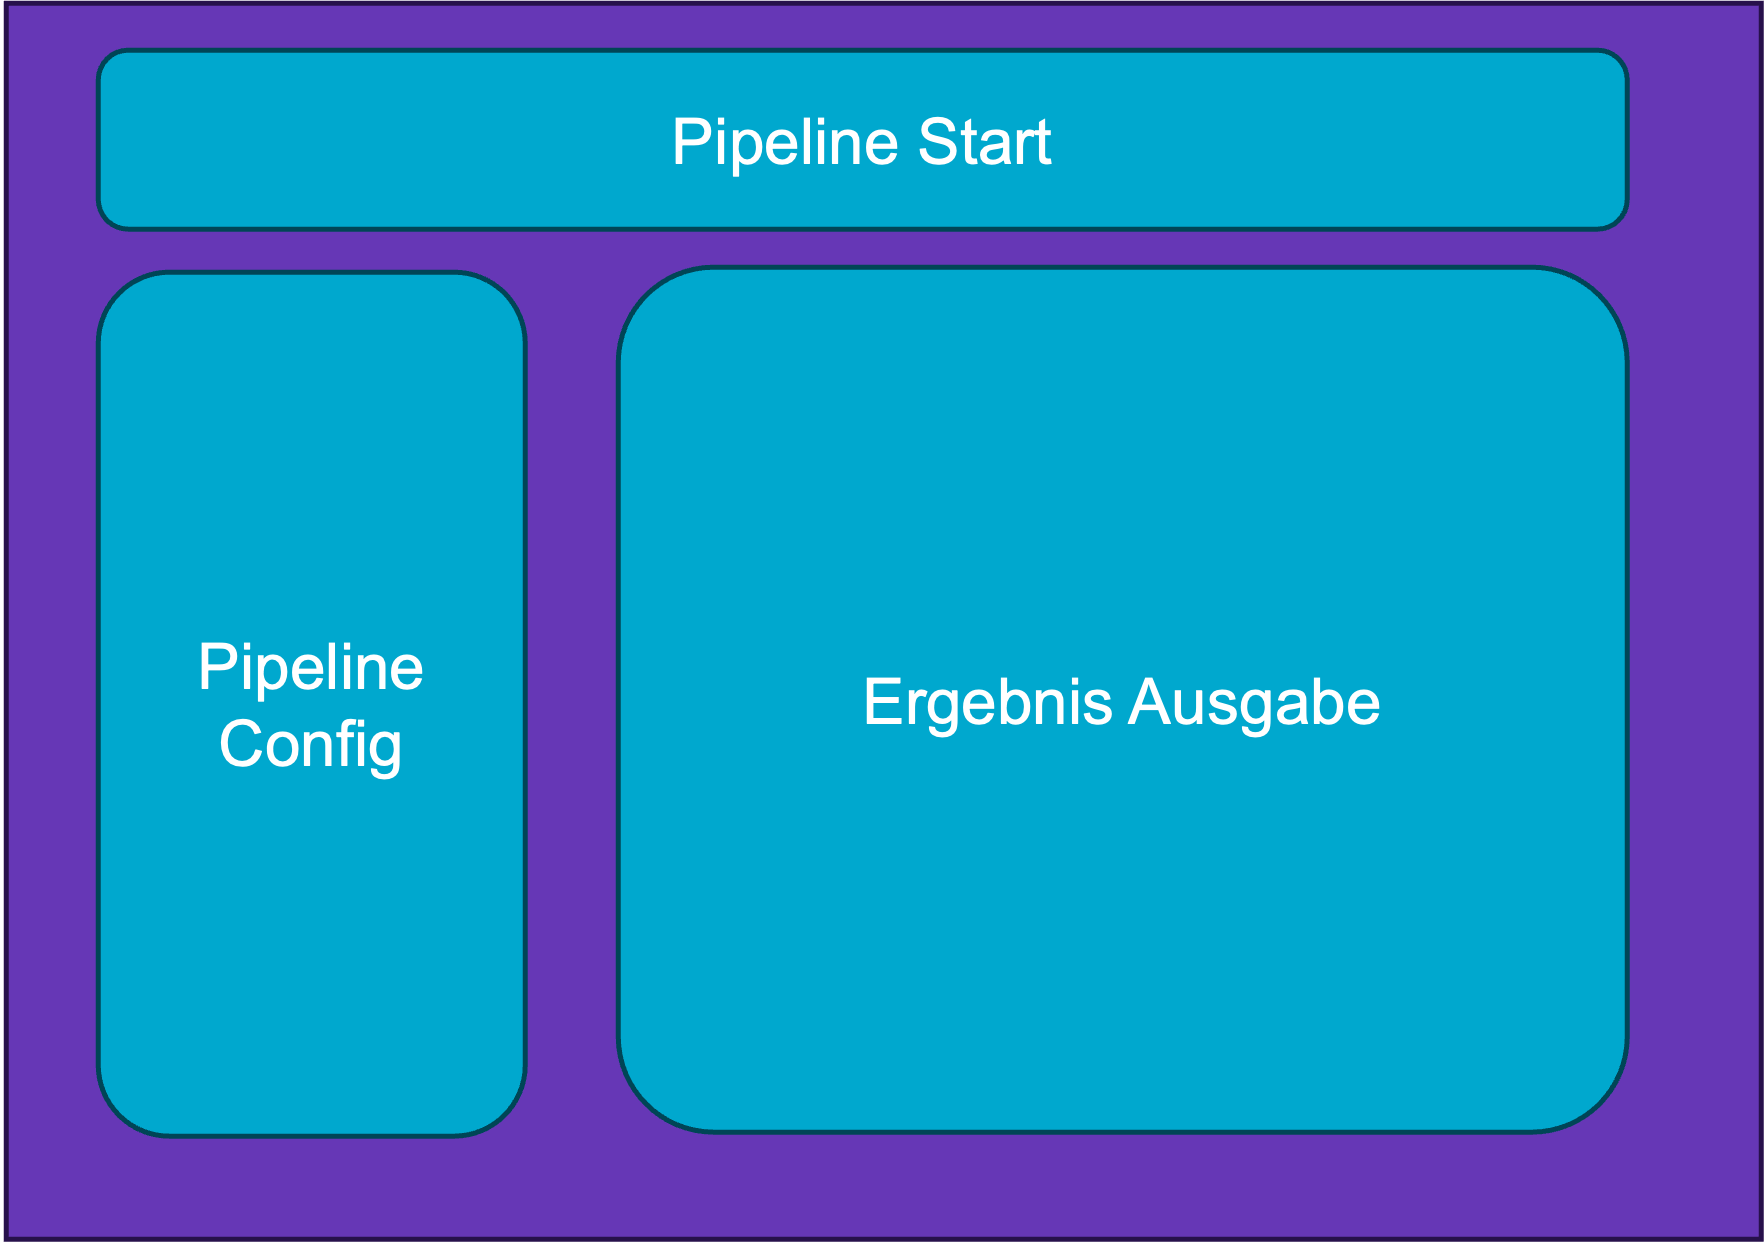
\includegraphics[width=0.7\textwidth]{img/ApplicationStructure.png}
    \caption{Aufbau der Demo-GUI.}
    \label{fig:application_structure}
\end{figure}

\begin{samepage}
Die GUI selbst ist nicht Teil der Pipeline, sondern nach dem MVC-Pattern aufgebaut. Sie nutzt lediglich die Pipeline-Architektur. Dadurch bleibt die Pipeline unabhängig von der GUI und kann auch an anderer Stelle wiederverwendet werden. Abbildung \ref{fig:gui_pipeline_interface} verdeutlicht diese Trennung: Die GUI steuert die Pipeline lediglich an und zeigt die Ergebnisse an, ohne direkt in deren Logik einzugreifen.

\begin{figure}[htbp]
    \centering
    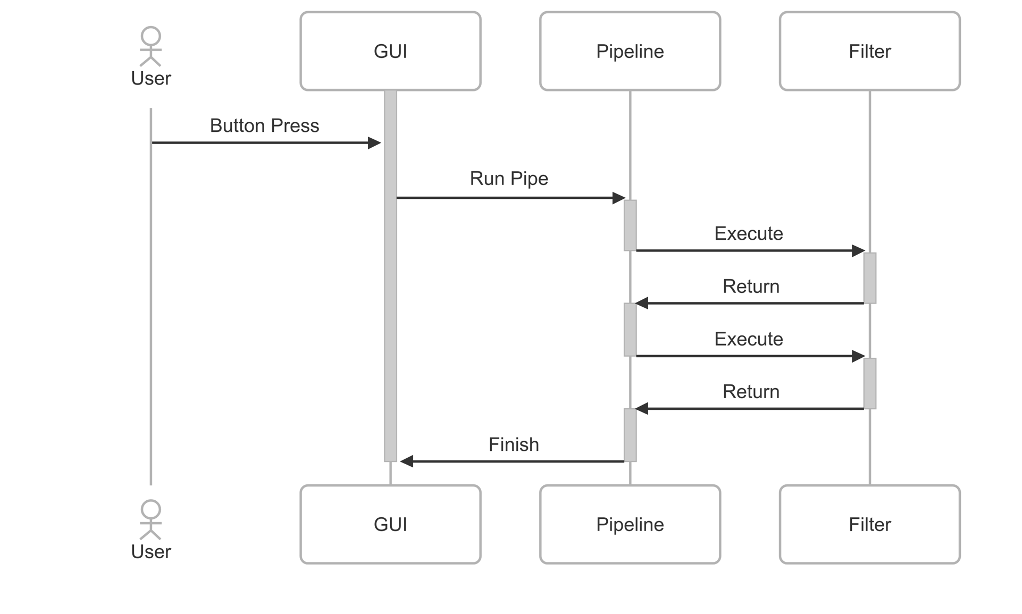
\includegraphics[width=0.7\textwidth]{img/GuiPipelineInterface.png}
    \caption{Kommunikation zwischen GUI und Pipeline.}
    \label{fig:gui_pipeline_interface}
\end{figure}
\end{samepage}

Wird die Pipeline über den „Open“-Button gestartet, öffnet sich zunächst ein Dateiauswahldialog, in dem der Benutzer die zu verarbeitende Datei auswählt. Dies ist der Einstiegspunkt in die Pipeline, die aus den folgenden Stufen besteht:

\begin{enumerate}
    \item \textbf{Loader:} In dieser ersten Stufe werden die Rohdaten von der Datenquelle (z.B. Bilddateien wie JPG, SVG etc.) eingelesen. Dazu gehört das Öffnen der Datei und das Parsen des Inhalts in eine interne Datenstruktur.
    \item \textbf{Transformer:} Auf die Daten werden Filter angewendet. Das können einfache Bildbearbeitungsschritte wie Drehen oder Spiegeln sein, aber auch komplexere Transformationen wie eine Bildanalyse mittels neuronaler Netze, um Merkmale zu extrahieren oder zu klassifizieren.
    \item \textbf{Tester:} Tester-Stufen prüfen, ob die Transformer korrekt angewendet wurden und die Ergebnisse den Erwartungen entsprechen.
    \item \textbf{Consumer:} Die verarbeiteten Ergebnisse werden gespeichert (z.B. in einer Datei oder Datenbank) oder an nachfolgende Systeme weitergegeben, etwa an die GUI zur Anzeige.
\end{enumerate}


\subsection{Implementierung der Pipeline-Steuerung: Die Wrapper-Klasse}
Die Implementierung einer Pipeline kann auf verschiedene Arten erfolgen, die sich hinsichtlich Flexibilität, Erweiterbarkeit und Entwicklungsaufwand unterscheiden. Gängige Ansätze sind:

\begin{itemize}
    \item \textbf{Direkte Implementierung im Code:} Die Reihenfolge der Stufen wird direkt im Code festgelegt. Das ist für kleine Pipelines einfach, wird aber bei wachsender Komplexität schnell unübersichtlich und schwer wartbar.
    \item \textbf{Konfigurationsbasierter Ansatz:} Die Pipeline-Struktur wird in einer externen Datei (z.B. YAML, JSON) definiert und zur Laufzeit geladen. Das bietet hohe Flexibilität und ermöglicht Anpassungen ohne Code-Änderungen, erfordert aber zusätzlichen Aufwand für das Parsen und Validieren der Konfiguration.
    \item \textbf{Wrapper-Klasse:} Eine eigene Klasse kapselt die Verwaltung der Stufen (Hinzufügen, Reihenfolge) und die Ausführung der Pipeline. Das fördert Struktur, Kapselung und Wiederverwendbarkeit.
\end{itemize}

Für die Beispielanwendung ist die Wrapper-Klasse der beste Ansatz. Sie trennt die Pipeline von der GUI, macht sie aber dennoch leicht zugänglich und ermöglicht dynamische Änderungen. Die zentrale Idee ist, eine Klasse (z.B. \texttt{Pipeline}) zu verwenden, die eine Liste von Pipeline-Stufen verwaltet. Jede Stufe wird als \texttt{Stage} bezeichnet und leitet von einer abstrakten Basisklasse ab. Dadurch muss jede konkrete Stufe die Methode \texttt{process} implementieren, was sicherstellt, dass alle Stufen einheitlich behandelt und von der Pipeline-Klasse aufgerufen werden können.

Die Wrapper-Klasse prüft zudem, dass nur gültige Stufen hinzugefügt werden. Dies geschieht durch Typ-Prüfungen, wie im folgenden Python-Codeausschnitt für die Methode \texttt{add\_stage} gezeigt:

\begin{figure}[htbp]
    \centering
    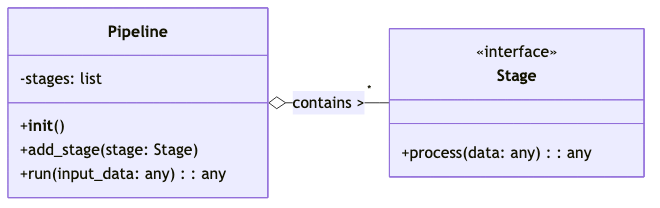
\includegraphics[width=0.8\textwidth]{img/wrapper.png}
    \caption{Klassendiagramm der Pipeline Wrapper-Klasse (\texttt{Pipeline}) und der abstrakten Stufenklasse (\texttt{Stage}).}
    \label{fig:wrapper}
\end{figure}

Damit Änderungen in einer Stage nur gezielt nachfolgende Stages beeinflussen, ist es sinnvoll, eine Datenklasse für den Datentransfer zwischen den Stages zu definieren. In der Beispielanwendung übernimmt dies die \texttt{PipeDataClass}. Jede Stage erwartet eine Instanz dieser Klasse als Parameter in der \texttt{process}-Methode und gibt eine modifizierte Instanz zurück. So bleiben die Daten zwischen den Stufen konsistent und nachvollziehbar.

Da die Demo eine Bildbearbeitung demonstriert, muss zwischen globalen und lokalen Änderungen unterschieden werden. Globale Änderungen betreffen das gesamte Bild (z.B. Drehen), während lokale Änderungen (z.B. Bounding Boxes von neuronalen Netzen oder Poster, die per Arucomarker platziert werden) nicht nachfolgende Filter beeinflussen sollen. Globale Änderungen greifen direkt auf das \texttt{base\_image\_from\_source} zu, während lokale Änderungen über \texttt{add\_optional\_layer} in eine Liste optionaler Layer eingetragen werden. Diese Layer werden in der Consumer-Stage zusammengeführt und als Ergebnis ausgegeben. Der Aufbau der \texttt{PipeDataClass} ist in Abbildung \ref{fig:pipeDataClass} dargestellt.

\begin{figure}[htbp]
    \centering
    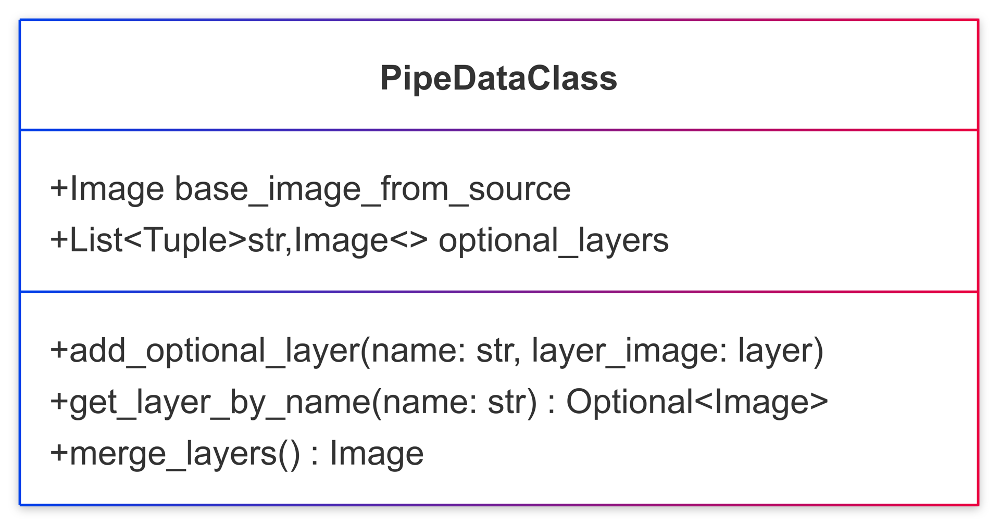
\includegraphics[width=0.8\textwidth]{img/PipeDataClass.png}
    \caption{Aufbau der PipeDataClass}
    \label{fig:pipeDataClass}
\end{figure}

\subsection{Factory Pattern zur dynamischen Komponentenauswahl}
Ein weiteres Entwurfsmuster, das die Pipeline-Architektur sinnvoll ergänzt, ist das Factory Pattern. Es dient dazu, Objekte zu erzeugen, ohne die konkrete Klasse im Voraus festlegen zu müssen. Die Verantwortung für die Objekterzeugung übernimmt eine spezialisierte Factory-Klasse oder -Methode.

Das Factory Pattern entkoppelt den aufrufenden Code von der konkreten Implementierung der zu erzeugenden Objekte. Die Factory entscheidet anhand der übergebenen Parameter oder des Kontexts, welche Unterklasse instanziiert und zurückgegeben wird.

\subsubsection{Anwendung im Datenlader}
Im Beispiel kommt das Factory Pattern beim Laden der Bilddaten zum Einsatz. Bilder liegen in unterschiedlichen Formaten vor, von pixelbasierten Formaten wie PNG und JPEG bis zu vektorbasierten wie SVG. Damit nachfolgende Stufen immer mit einheitlichen Eingangsdaten arbeiten können, erfolgt eine Transformation auf ein Standardformat (hier: pixelbasiert). Anstatt die Logik zur Erkennung und Verarbeitung jedes Formats direkt in die Pipeline-Stufe einzubauen, wird eine \texttt{LoaderFactory} verwendet.

Der Ablauf ist typischerweise wie folgt:
\begin{enumerate}
    \item Eine vorherige Pipeline-Stufe oder der Initialaufruf übergibt den Dateipfad oder eine Kennung der zu ladenden Daten an die zuständige Stufe.
    \item Diese Stufe delegiert die Erzeugung des passenden Ladeobjekts an die \texttt{LoaderFactory} und übergibt relevante Informationen (z.B. Dateipfad oder -format).
    \item Die \texttt{LoaderFactory} analysiert die Informationen (z.B. Dateiendung wie \texttt{.png} oder \texttt{.svg}).
    \item Basierend darauf instanziiert die Factory das passende Ladeobjekt (z.B. \texttt{PNG\_Loader} oder \texttt{SVG\_Loader}), das eine gemeinsame Schnittstelle (\texttt{DataLoader}) implementiert.
    \item Die Factory gibt das erzeugte Ladeobjekt an die aufrufende Pipeline-Stufe zurück.
    \item Die Pipeline-Stufe verwendet das Ladeobjekt, um die Daten zu laden, ohne die konkrete Implementierung kennen zu müssen.
\end{enumerate}

Abbildung \ref{fig:loaderFactory} zeigt diesen Entscheidungsprozess. Die Factory prüft das angeforderte Format und wählt den passenden Loader aus. Ist kein passender Loader registriert oder existiert die Datei nicht, wird ein Fehler ausgelöst oder ein Null-Objekt zurückgegeben. Für die Pipeline ist dieser Prozess transparent – der Loader verhält sich wie eine normale Stage-Klasse.

\begin{figure}[htbp]
    \centering
    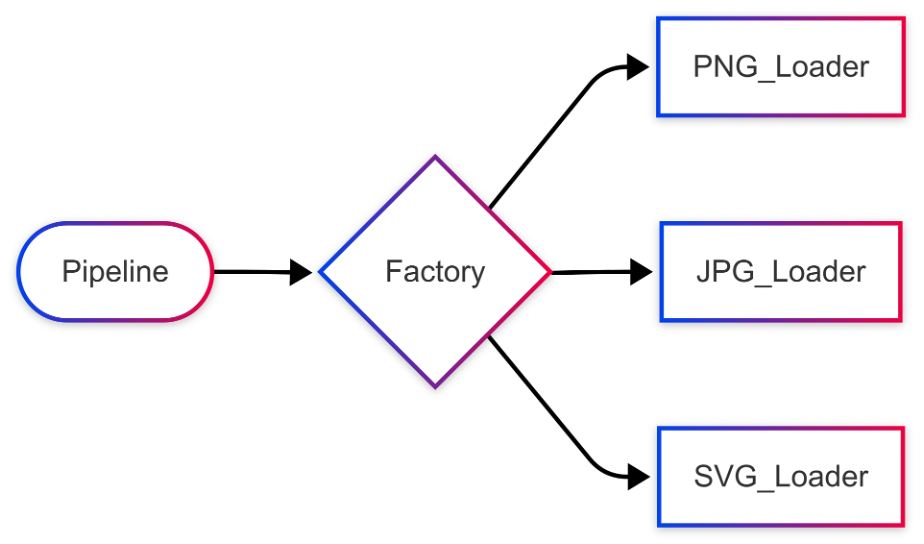
\includegraphics[width=0.8\textwidth]{img/PipelineFactory.png}
    \caption{Entscheidungsdiagramm der LoaderFactory zur Auswahl des passenden Datenladers basierend auf dem Dateiformat.}
    \label{fig:loaderFactory}
\end{figure}

\subsubsection{Vorteile des Factory Patterns in der Pipeline}
Das Factory Pattern bietet in diesem Kontext mehrere Vorteile:

\begin{itemize}
    \item \textbf{Entkoppelung:} Die Pipeline-Stufe, die Daten lädt, ist von den konkreten Ladeimplementierungen entkoppelt und arbeitet nur mit der Factory und der abstrakten Schnittstelle.
    \item \textbf{Flexibilität und Erweiterbarkeit:} Neue Dateiformate können einfach durch Implementieren einer neuen \texttt{DataLoader}-Unterklasse und Anpassen der Factory unterstützt werden, ohne die Pipeline-Stufe zu ändern.
    \item \textbf{Zentralisierung der Erzeugungslogik:} Die Entscheidung, welcher Loader wann erstellt wird, ist an einer zentralen Stelle gebündelt.
    \item \textbf{Verbesserte Testbarkeit:} Loader-Klassen und Factory können isoliert getestet werden.
    \item \textbf{Wiederverwendbarkeit:} Factory und Loader-Klassen können auch in anderen Anwendungen oder Projekten genutzt werden.
\end{itemize}

Zusammengefasst verbessert das Factory Pattern die Struktur der Pipeline, indem es die Erzeugung von Komponenten wie Datenladern flexibler, wartbarer und erweiterbarer macht.

\subsection{Pipeline mit Checkpoints}
Ein Nachteil der klassischen Pipeline-Architektur ist ihre lineare Struktur: Die Verarbeitung erfolgt in fester Reihenfolge, und es ist schwierig, den Prozess zu unterbrechen oder an einem bestimmten Punkt neu zu starten. Das kann problematisch sein, wenn Fehler auftreten oder die Verarbeitung lange dauert und der Benutzer einzelne Stufen verändern möchte.

Um dieses Problem zu lösen, können Checkpoints eingesetzt werden. Sie ermöglichen es, den Zustand der Pipeline zu einem bestimmten Zeitpunkt zu speichern, sodass die Verarbeitung später an dieser Stelle fortgesetzt oder erneut durchgeführt werden kann. Das ist besonders nützlich, wenn z.B. ein neuronales Netz ein Bild analysiert und dieser Schritt viel Zeit beansprucht.

Wie oft und an welcher Stelle Checkpoints erzeugt werden, entscheidet der Entwickler. Im Demobeispiel wird vor jeder Stage im Transformer- oder Tester-Bereich ein Checkpoint erzeugt. So kann der Benutzer jederzeit Änderungen an beliebigen Teilen der Pipeline vornehmen. Durch Drücken des Update-Buttons in der GUI (siehe Abbildung \ref{fig:gui_pipeline_interface}) wird die Pipeline an der zuletzt unveränderten Stelle neu gestartet.

\newpage
\begin{thebibliography}{99}
\bibitem{richards2020} Mark Richards und Neal Ford. \textit{Handbuch Moderner Softwarearchitektur: Architekturstile, Patterns und Best Practices}. O'Reilly Verlag GmbH & Co. KG, 2020.
\bibitem{uqcloud_pipeline} CSSE6400. \textit{Pipeline Architecture}. \url{https://csse6400.uqcloud.net/handouts/pipeline.pdf}
\bibitem{oreilly_python_pipes} O'Reilly. \textit{Software Architecture with Python: Pipe and Filter architectures}. \url{https://www.oreilly.com/library/view/software-architecture-with/9781786468529/ch08s04.html}
\bibitem{researchgate_parallel_pipes} ResearchGate. \textit{The Pipes and Filters Pattern: A Functional Parallelism Architectural Pattern for Parallel Programming}. \url{https://www.researchgate.net/publication/221034471_The_Pipes_and_Filters_Pattern_A_Functional_Parallelism_Architectural_Pattern_for_Parallel_Programming}
\bibitem{azure_pipes_filters} Explore Azure Cloud. \textit{Pipes and Filters Pattern in Azure - Part 1}. \url{https://exploreazurecloud.com/pipes-and-filters-pattern-in-azure-part-1}
\bibitem{projectpro_etl_usecases} ProjectPro. \textit{Top ETL Use Cases for BI and Analytics: Real-World Examples}. \url{https://www.projectpro.io/article/etl-use-cases/768}
\bibitem{researchgate_etl_dist} ResearchGate. \textit{Distributed ETL Architecture for Processing and Storing Bigdata}. \url{https://www.researchgate.net/publication/382522030_Distributed_ETL_Architecture_for_Processing_and_Storing_Bigdata}
\bibitem{wso2_eip} WSO2 Docs. \textit{Pipes and Filters EIP}. \url{https://wso2docs.atlassian.net/wiki/spaces/EIP/pages/48791632/Pipes+and+Filters}
\bibitem{acceldata_streaming} Acceldata. \textit{Mastering Streaming Data Pipelines for Real-Time Data Processing}. \url{https://www.acceldata.io/blog/mastering-streaming-data-pipelines-for-real-time-data-processing}
\bibitem{dagster_frameworks} Dagster. \textit{Data Pipeline Frameworks: Key Features & 10 Tools to Know in 2024}. \url{https://dagster.io/guides/data-pipeline/data-pipeline-frameworks-key-features-10-tools-to-know-in-2024}
\bibitem{packt_cpp_architecture} Packt. \textit{Software Architecture with C++: Architectural and System Design}. \url{https://www.packtpub.com/fr-cy/product/software-architecture-with-c-9781838554590/chapter/architectural-and-system-design-6/section/pipes-and-filters-pattern-ch06lvl1sec35}
\bibitem{dagster_data_pipeline} Dagster. \textit{Data Pipeline}. \url{https://dagster.io/guides/data-pipeline}
\end{thebibliography}

\end{document}
